\documentclass[11pt,letterpaper]{article}
\usepackage{fullpage}
\usepackage[top=2cm, bottom=4.5cm, left=2.5cm, right=2.5cm]{geometry}
\usepackage{amsmath,amsfonts,amssymb}
\usepackage{lastpage}
\usepackage[inline]{enumitem}
\usepackage{fancyhdr}
\usepackage{mathrsfs}
\usepackage{xcolor}
\usepackage{graphicx}
\usepackage{hyperref}
\hypersetup{colorlinks=true, linkcolor=blue, linkbordercolor={0 0 1}}

\renewcommand{\arraystretch}{1.75}

\setlength{\parindent}{0.0in}
\setlength{\parskip}{0.05in}

\pagestyle{fancyplain}
\lhead{Brad Cownden}
\chead{}
\rhead{April 2, 2020}
\cfoot{\small\thepage}
\headsep 36pt

\begin{document}
\vspace{.2in}
\begin{center}
    {\bf GPU Solutions for PSCAD: IT17112}
\end{center}

	\vspace{.25in}

\begin{tabular}{| p{0.2\textwidth} | p{0.75\textwidth} |}
	\hline
	Reporting Period & April 2, 2020 - April 9, 2020 \\ \hline

	Activities & \begin{enumerate*}
	\item[\tiny\textbullet] Ran new sparse matrix code on entire \emph{Province} data set and recorded GPU solve time per time step
	\end{enumerate*} \\ \hline

	Issues & \begin{enumerate*}
	\item[\tiny\textbullet] None
	\end{enumerate*} \\ \hline

	Milestones \newline Accomplished & \begin{enumerate*}
	\item[\tiny\textbullet] First run through of entire \emph{Province} data set
  \end{enumerate*} \\ \hline

	Milestones Not \newline Accomplished & \begin{enumerate*}
	\item[\tiny\textbullet] None
	\end{enumerate*} \\ \hline

	Next Week's \newline Milestones & \begin{enumerate*}
	\item[\tiny\textbullet] Load \& run matrix solving on U of W GPU resources
	\end{enumerate*} \\ \hline

	Forwarded Issues & \begin{enumerate*}
	\item[\tiny\textbullet] None
	\end{enumerate*} \\ \hline
\end{tabular}

\begin{figure}[h!]
  \centering
  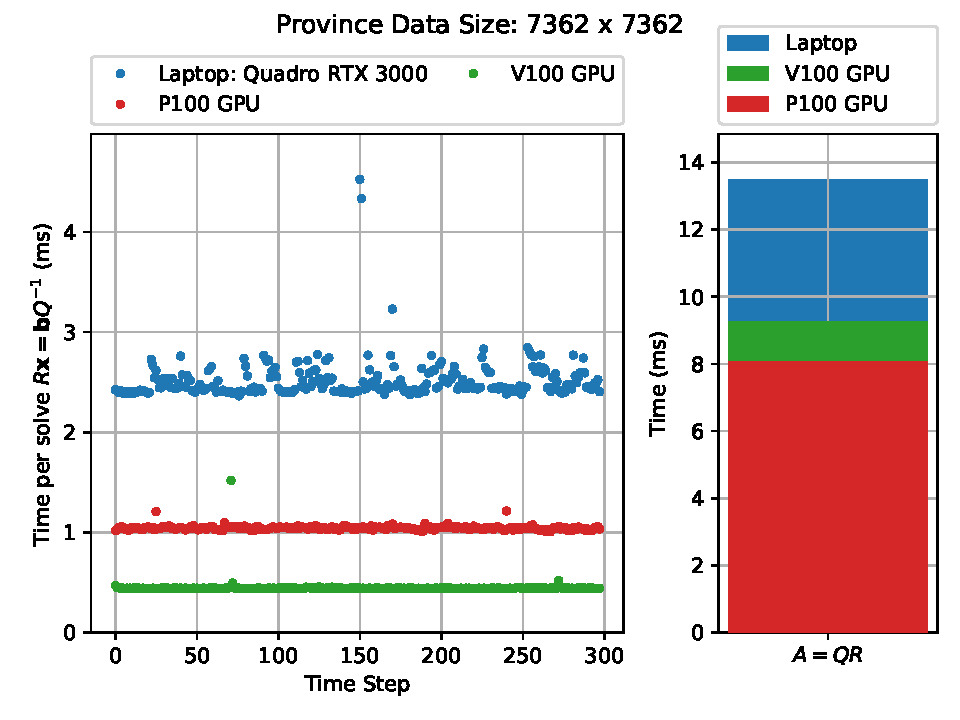
\includegraphics[width=0.75\textwidth]{C:/Users/bradc/Documents/MHI/Output/FullTimings}
  \caption{Timing for solving for $\mathbf{x}(t_0)$ after matrix factorization for the entire \emph{Province} data set.}
  \label{}
\end{figure}

\end{document}
